\chapter{Implementation}
\index{Implementation%
@\emph{Implementation}}%

\section{Overview}
Speakur\index{Speakur} is an HTML5\index{HTML!HTML5} web application that uses the Polymer\index{Polymer} framework's Web Components\index{Web Components} architecture.
It is primarily a client side application with no dedicated server component other than Firebase\index{Firebase}.
It is delivered as a single Custom Element\index{Custom Elements}, \tcode{<speakur-discussion>}\index{<speakur-discussion>}.
You import the tag with \tcode{<link rel=import href=...>} to make it available to place on the page. 
This element has a data-bound\index{data-bound template} \tcode{<template>}\index{<template>} that provides the element's visual representation (shadow DOM).
Actually, a custom element's representation, or logical DOM\index{Logical DOM}, may consist of both encapsulated shadow DOM\index{Shadow DOM} as well as light DOM\index{Light DOM} that is supplied by the \textit{user} of the custom element and \textit{projected} into the shadow DOM as discussed in section~\ref{bg:shadowdom}.
In Speakur's case, the discussion forum is self-contained in terms of content; light DOM is not needed or used in the top-level element.
Speakur's\index{Speakur} options or parameters are controlled with attributes\index{HTML!attributes}:

\begin{lstlisting}[language=HTML5,caption=
{Using HTML attributes to set Speakur options},label=l:options1,captionpos=below]
 <speakur-discussion
   firebaseLocation="https://speakur-demo.firebaseio.com"
   xtitle="This is the thread's (initial) title."
   href="demo1"
   initiallyOpen="true"
   allowAnonymous="true">
 </speakur-discussion>
\end{lstlisting}

%Speakur is subdivided into a number of components which abstract\index{abstraction} behavior and encapsulate\index{encapsulation} the implementation details.
%These components use Polymer\index{Polymer} data bindings\index{data-bound template} to reflect state changes between the user interface and local and remote data models.
%Security is handled by Firebase authorization rules.
%Responsive design with \tcode{flex} and \tcode{@media} attributes adjusts the interface automatically for desktop and mobile users.
%Speakur takes advantage of data bindings to offer localization features that instantly update when the language preference is changed.

\section{Layout and structure}
\label{sec:layout}

Structurally, Speakur\index{Speakur} consists of JavaScript\index{JavaScript}, HTML, and CSS\index{CSS} files, along with a few other resource types like images and JSON\index{JSON} language files. 
All of the these internal resources and components are hidden from consumers who only have to import and place the main \tcode{<speakur-discussion>}\index{<speakur-discussion>} element as discussed in section~\ref{publishing} below.
The rest of the components are brought in by imports inside \tcode{<speakur-discussion>}\index{<speakur-discussion>}.

\begin{table}\centering
\ra{1.3}
\begin{tabular}{@{}lp{8cm}@{}}
\toprule
Name & Function \\
\midrule
\textbf{Structural~containers}\\
\tcode{<speakur-discussion>} & Top-level public component. \\
\tcode{<speakur-thread-view>} & Container for the comments displayed in an entire thread. \\
\tcode{<speakur-card>} & Provides a Material Design\index{Material Design} `card' container. \\
\tcode{<speakur-post-set>} & A container for a list of posts such as replies to a specific post. \\
\\
\textbf{Logical~services}\\
\tcode{<firebase-element>}\index{<firebase-element>} & Polymer's\index{Polymer} Web Component wrapper around Firebase\index{Firebase}. \\
\tcode{<speakur-base>} & Base-class for most other Speakur components. \\
\tcode{<speakur-i18next>} & My Web Component wrapper around the i18next library~\cite{i18nextcontributors2015}. \\
\tcode{<speakur-profile>} & Users' session data and preferences. \\
\tcode{<speakur-post-vote>} & Controller for voting posts up or down. \\
\\
\textbf{User~Interface}\\
\tcode{<speakur-compose>} & Composing replies and posts. \\
\tcode{<speakur-post>} & Displays a single user post/comment. \\
\tcode{<speakur-login-button>} & Login/logout button and dropdown. \\
\tcode{<speakur-theme>} & Base class for all themes, mainly CSS rules. \\
\tcode{<speakur-theme-blue>} & A specific theme. \\
\tcode{<speakur-dialog-profile>} & Dialog to edit user preferences. \\
\tcode{<speakur-lang-select>} & Dropdown to choose the UI language. \\
\bottomrule
\end{tabular}
\caption{Partial list of Speakur's internal components.}
\label{table:speakurcomponents}
\end{table}

Internally, Speakur\index{Speakur} is composed of a number of sub-components, a partial list of which is found in Table~\ref{table:speakurcomponents}. 
These components are listed in three broad categories: structural containers, 
logical services, 
and user interface\index{user interface (UI)} elements.
The structural elements provide a container and abstraction layer for a group of related child elements.
For example, \tcode{<speakur-card>} provides a Material Design-styled\index{Material Design} generic `card' consisting of a styled header, body, and footer.
These containers may have certain visible elements such as lines around their border, but most of their representation comes from the components inside.

The logical service elements do not have any visual representation at all.
They perform data-related services, provide purely abstract APIs, and wrap external libraries.
For example, the Firebase\index{Firebase} client library is a general purpose JavaScript library, and is not specifically adapted to Web Components or custom elements.
Therefore it is often useful to provide a custom element wrapper around a non-WC-aware library.
For this reason the Polymer project maintains \tcode{<firebase-element>}\index{<firebase-element>} as a wrapper around the main Firebase library~\cite{polymercontributors2015-c}.
Within Speakur, each component gets its data either directly from its own internal \tcode{<firebase-element>}\index{<firebase-element>}, or else from a data binding from an immediate parent element that has its own \tcode{<firebase-element>}\index{<firebase-element>}.

Figure~\ref{f:file_layout} shows a partial listing of the internal component files.
One of these is abstraction layer for an internationalization\index{internationalization} library.
Following the \tcode{<firebase-element>}\index{<firebase-element>} example, 
I created a simple custom element wrapper around the \textbf{i18next} 
JavaScript\index{JavaScript} library~\cite{i18nextcontributors2015}.
This wrapper is called \tcode{<speakur-i18next>}\index{<speakur-i18next>}. 
It tells i18next where to find Speakur's translation files and creates a Polymer \textit{filter} to perform translations from data-bound templates\index{data-bound template}. 
See section~\ref{sec:i18n} below for details.
Logical elements are also used to provide abstract `controllers' 
(in the MVC\index{model-view-controller} sense), 
facades, pseudo-OOP\index{object oriented programming (OOP)} base classes and other design patterns.

\begin{figure}[htb]
	\centerline{
	\begin{subfigure}[b]{0.48\textwidth}
		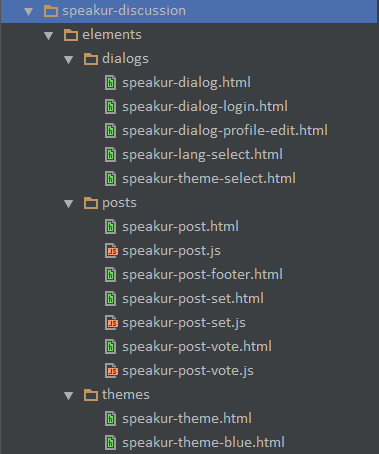
\includegraphics[width=\textwidth]{images/file_layout_a.png}
	\end{subfigure} %
	\begin{subfigure}[b]{0.48\textwidth}
		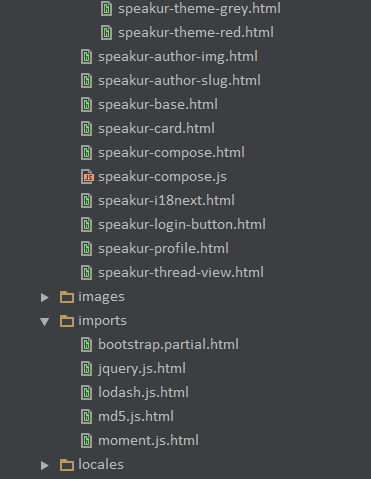
\includegraphics[width=\textwidth]{images/file_layout_b.png}
	\end{subfigure} %
	}
	\caption{Internal elements file layout (partial).}
	\label{f:file_layout}
\end{figure}

In addition to structural and logical elements, 
Speakur has a number of user interface (UI)\index{user interface (UI)} custom elements to do things like display an individual user post or show the post composition editor.
Elements are also reused extensively in different contexts; 
for example \tcode{<speakur-post>} is used for a `live editor preview' inside \tcode{<speakur-compose>} as well as for showing posts in the main \tcode{<speakur-thread-view>.}

Some of Speakur's internal components like \tcode{<speakur-theme>} are also `base classes' for other elements
in a way that is similar but not identical to classes in object oriented programming (OOP)\index{object oriented programming (OOP)}\footnote{Note that JavaScript\index{JavaScript} itself is \textit{prototype}-based\index{prototype (JavaScript)} and does not have traditional classes or inheritance. 
Similar behavior is obtained by using regular object instances (instead of classes) as the prototype for instantiating new objects.}. 
Although composition or \textit{has-a} relationships are generally preferred, inheritance or \textit{is-a} relationships can make sense when you truly want to be able to substitute one instance for another interchangeably.

\section{Database design}
\label{sec:database}

Speakur uses Firebase for NoSQL\index{NoSQL}-style database storage.
Traditional relational databases\index{relational database} (SQL\index{SQL}) have emphasized data normalization\index{normalization (database)} -- the removal of informational redundancies from databases such that a given \textit{fact} is only recorded in a single place.
While this helps ensure data integrity, it can adversely affect query time and scalability as additional joins are required to bring in the necessary facts.
One of the defining characteristics of the NoSQL movement is denormalization\index{denormalization}
--- that is, the principle of eliminating redundancy is sacrificed in order to gain performance~\cite{sadalage2012}.
Facts can be defined in more than one place to speed up queries.

For example, some information about a post's author 
such as their public username, id, and photo url is saved inside each post they write 
so that it's not necessary to look up this information separately just to display the post.
One consequence of this is that changing your public name doesn't retroactively change the name on all of your previous posts, just new posts going forward.
Certainly, if that name updating was deemed necessary per business requirements it could be accomplished.

% p{8cm}
\begin{table}\centering
\ra{1.3}
\begin{tabular}{@{}lll@{}}
\toprule
Table Name & Function & Key Structure \\
\midrule
\tcode{admins} & Administrator authorizations & \tcode{\$uid} \\
\tcode{posts} & User posts & \tcode{\$parent->\$child} \\
\tcode{postvotes} & Public vote counts for posts & \tcode{\$parent->\$child} \\
\tcode{profile} & User data and preferences & \tcode{\$uid} \\
\tcode{threads} & Discussion thread definitions & \tcode{\$threadId} \\
\tcode{uservotes} & User votes for posts & \tcode{\$uid->\$parent->\$child} \\
\bottomrule
\end{tabular}
\caption{Speakur's database tables.}
\label{table:speakurtables}
\end{table}

The logical interface presented by Firebase\index{Firebase} resembles a single JavaScript\index{JavaScript} object which can contain other objects and lists nested up to 32 levels deep~\cite{firebasecontributors2015}.
A JavaScript object is fundamentally a \tcode{key->value} mapping, also known as a hash map or (in Python\index{Python language}) as a dictionary.
Although this nested object structure doesn't correspond exactly to traditional relational database\index{relational database} (SQL\index{SQL}) tables, 
it is convenient to refer to the top (first) level of nested objects as ``tables''.
The leaf node objects are ``records'' with data fields, and the intermediate objects are keys within the table.
Like most NoSQL databases, Firebase is forgiving with regard to structure and fields; 
a given record is not guaranteed to follow any particular structure unless this is required by the security and validation rules.

\begin{figure}[htb]
\centering
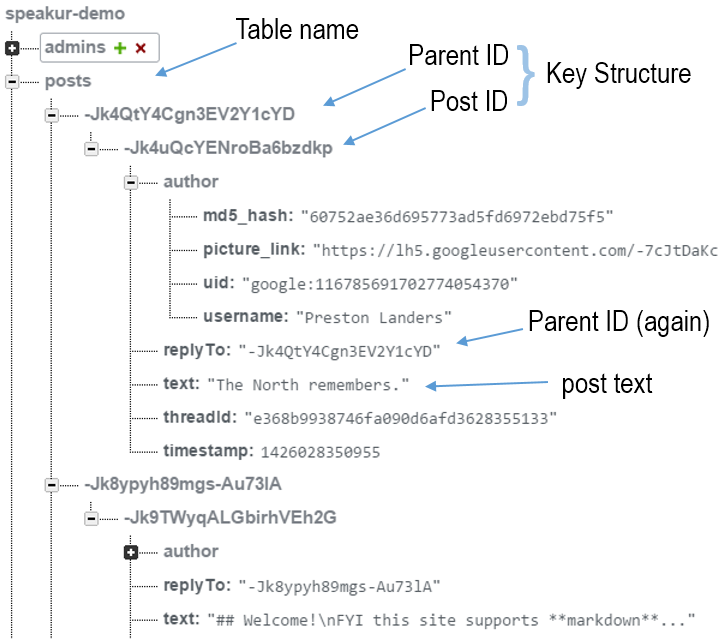
\includegraphics[width=0.93\textwidth]{images/firebase_admin_posts_b.png}
\caption{Structure of the \tcode{posts} table.}
\label{f:firebase_admin_posts}
\end{figure}

The key structure column in Table~\ref{table:speakurtables} signifies the meaning of the keys underneath a table. 
For example, the main \tcode{posts} table has a \tcode{\$parent->\$child} key structure, 
which means that the first layer of keys beneath \tcode{posts} are post \textit{parent} ids, 
meaning the id of the post that this post is a reply to, 
or the thread id in the case of a `top-level' post.
The next nested object down is the \textit{child} id, 
or the id of the actual post itself, 
and the keys under that are the `fields' of the table, 
such as the \tcode{text} and \tcode{replyTo} values.
Figure~\ref{f:firebase_admin_posts} shows Firebase's administrative view of the database where the \tcode{posts} table is expanded, 
showing the parent and child id layers, 
and the actual post nested within.
Deeply nested data structures are not good for scalability; 
relatively flat tables are best~\cite{firebasecontributors2015,sadalage2012}.
The key structure will become important when we apply security rules in section~\ref{sec:security}.


In addition to denormalizing\index{denormalization} the data as necessary, sometimes it is convenient for security reasons to 
keep related bits of data in separate tables in order to apply different security rules.
For instance, we want users to be able to modify a post's vote count without being able to modify the post itself.
The nested and denormalized\index{denormalization} structure of the tables helps ensure that we only fetch what we need, when we need it.
The flip side is that we need to be aware of these data duplications and update them as necessary, 
which can be difficult in a more sophisticated application.
But in the post vote count example, even if a malicious user sets a false count on the globally-visible value,
we can always recalculate the true count later using the individual user vote records.

\section{Component synchronization}
\label{sec:sync}

Speakur\index{Speakur} consists of a number of Polymer\index{Polymer} components which break down the problem of presenting a discussion forum into smaller tasks.
Some of these components are listed in Table~\ref{table:speakurcomponents}.
They form a hierarchy with \tcode{<speakur-discussion>}\index{<speakur-discussion>} at the top (root). 
Figure~\ref{f:component_layout} illustrates this, with many components omitted for brevity.

\begin{figure}[htb]
	\centerline{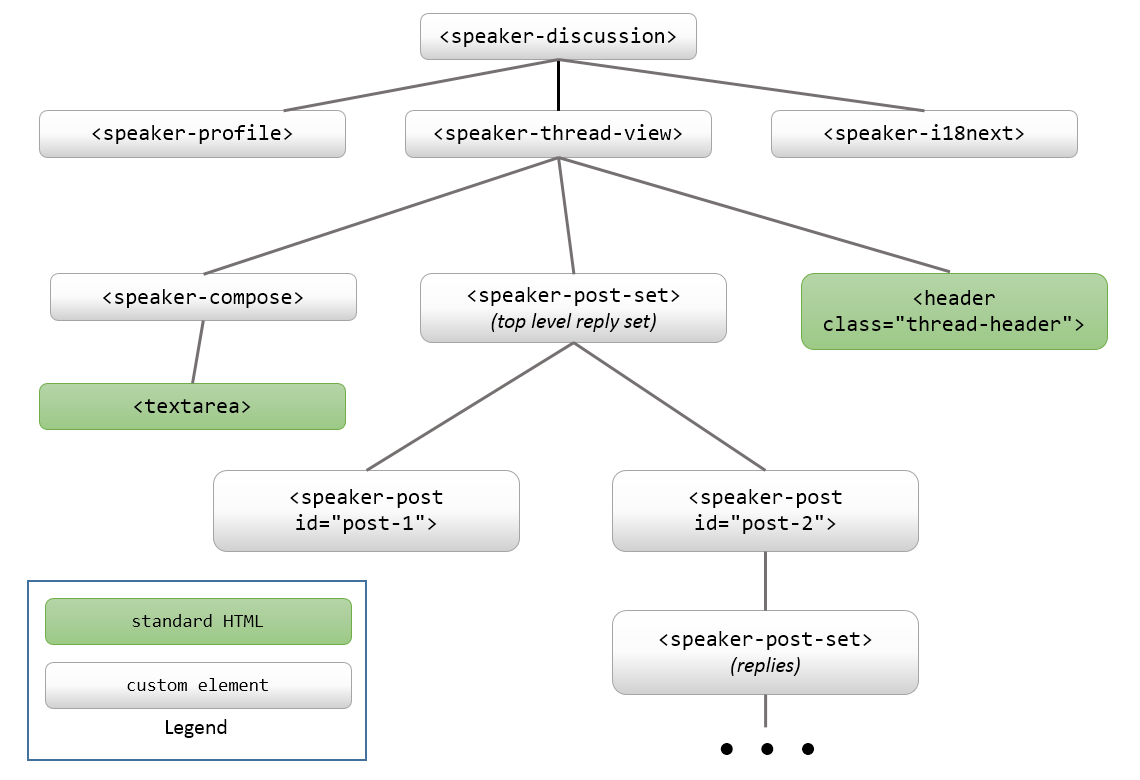
\includegraphics[width=6in]{images/components.png}}
	\caption{Speakur component hierarchy (partial).}
	\label{f:component_layout}
\end{figure}

The general data flow is that bindings carry information \textit{down} from parent to child, and changes flow \textit{up} in the form of events and observed mutations.
Two-way bindings are possible in that a child element can modify a bound variable and the value would be reflected in the parent and vice-versa, 
but in some scenarios this makes it difficult to determine an `authoritative' value 
or causes other circularity problems.
For this reason, bindings should be used one-way across component lines,
but two-way bindings are useful within a component to update its `data model' automatically from user input~\cite{polymercontributors2015-b}.

Each component keeps its own \tcode{<firebase-element>}\index{<firebase-element>} to pull data from Firebase\index{Firebase} as needed,
or in some cases the relevant object is passed in as a binding from a parent element that has its own \tcode{<firebase-element>}\index{<firebase-element>}.
This keeps database specific knowledge localized to each component, helping it ``be composable''.
Speakur\index{Speakur} as a whole doesn't know or care what storage solution its individual components use, whether Firebase\index{Firebase} or another API\index{API}.

\subsection{Data bindings and events}
\label{sec:databindings}
From an MVC\index{model-view-controller} viewpoint, a Polymer element with instance variables \textit{is} the `model'.
The element's data-bound\index{data-bound template} \tcode{<template>}\index{<template>} is the `view', 
and the JavaScript\index{JavaScript} code is the `controller'.
Data bindings carry data information down from parent to child while DOM\index{DOM} events\index{event notification} propagate upwards.

Using \tcode{<firebase-element>}\index{<firebase-element>} isolates each component from direct interaction with the general purpose Firebase\index{Firebase} JavaScript library
and ties the database directly into the Polymer\index{Polymer} data binding system.
Persisting changes is incredibly easy; 
writing a new value to a variable not only saves it to the database but pushes the change
to all other `subscribers' --- whoever is viewing that post or other object at the time.
The \tcode{data=} attribute on 
\tcode{<firebase-element>}\index{<firebase-element>}
allows binding a variable in a component to a remote database object:

\begin{lstlisting}[language=HTML5,caption={Binding the \tcode{post} variable to a database record.},label=l:fb_bind,captionpos=below]
<!-- from speakur-post.html -->
<firebase-element
   data="{{ post }}"
   location="{{ fbLocation(firebaseLocation, 'posts', parentId, postId) }}">
</firebase-element>
\end{lstlisting}

In the example above, 
the data retrieved by the \tcode{<firebase-element>}\index{<firebase-element>}
is bound by the \tcode{\{\{ \}\}} operators to the component's \tcode{post} variable. 
Any changes to this database object, 
whether locally or remotely initiated,
will be reflected in the \tcode{post} variable
and any associated data-bound\index{data-bound template} \tcode{<template>}\index{<template>}s, 
and vice-versa.
Note that the \tcode{location=} attribute (the database source URL for this \tcode{<firebase-element>}\index{<firebase-element>})
is bound to an expression which finds the location with the \tcode{fbLocation} method.
Any changes in the variables \tcode{firebase\-Location}, \tcode{parentId} or \tcode{postId} will cause \tcode{fbLocation} to be recomputed,
which could in turn cause \tcode{post} to pull from a different location.
Note that \tcode{location=} has the same structure as the resource path in the \tcode{DELETE} example from Listing~\ref{l:rest_delete}.

DOM events carry state changes up from children to elements above it.
Polymer provides the \tcode{fire()} method to trigger a named event with extra data attached.
This is a convenience wrapper since it can be done with pure JavaScript\index{JavaScript}.
An example of using \tcode{fire()} can be found in the language selection dialog from Figure~\ref{f:lang}.
The language selection UI is handled in the \tcode{<speakur-lang-select>} component,
which is only concerned with presenting the language chooser and not with handling the actual localization,
reinforcing separation of concerns.
When the user selects a new language it fires an event that bubbles up to the top level \tcode{<speakur-discussion>} element:

\begin{lstlisting}[language=JavaScript,caption={Firing a language change event.},label=l:fire_event,captionpos=below]
// from speakur-lang-select.js
domReady: function () {
    // listen for core-select event fired by the dropdown menu
    this.$.menu.addEventListener('core-select', function (e) {
        if (e.detail.isSelected) {
            var oldLocale = this.locale;
            var newLocale = e.detail.item.id;
            
            // Tell container(s) the language selection changed
            this.fire('speakur-locale-change', 
               {oldLocale: oldLocale, newLocale: newLocale});
        }
    });
}
\end{lstlisting}

A handler in the top level container (\tcode{<speakur-discussion>}\index{<speakur-discussion>}) responds to this named event (\tcode{speakur-locale-change}) and tells the
internationalization\index{internationalization} component to update the language.
This in turn sets the \tcode{\textbf{lc}} (locale) property in the base element.
This property is then used in translation expressions as discussed in section~\ref{sec:i18n} below.

\subsection{Data-bound templates}
Speakur translates internal variables (the model) into visible output with the use of data-bound templates\index{data-bound template}.
This is similar in effect to the model-view-controller\index{model-view-controller} design pattern.
As mentioned above, the custom element itself is the `model' and its \tcode{<template>}\index{<template>} is the view.
This allows embedding variables directly in the HTML\index{HTML} representation of a component as shown in Listing~\ref{l:dbtemplate} and here:

\begin{lstlisting}[language=HTML5,caption={User interface control with data bindings (edit post link).},label=l:bind_ui,captionpos=below]
<!-- from speakur-post-footer.html -->
<div on-click="{{editPost}}" hidden?=
    "{{!canEditPost(post, globals.profile, globals.isAdmin)}}">
  {{ "Edit" | $$(lc) }}
</div>
\end{lstlisting}

There are three data bindings with \tcode{\{\{ \}\}} in Listing~\ref{l:bind_ui}:
\begin{enumerate}
\item The \tcode{hidden?=} attribute (provided by Polymer\index{Polymer}) binds to \tcode{canEditPost} to determine if the Edit link should be shown under a post. 
In other words, is this user allowed to edit this post? If not, hide this Edit \tcode{<div>}.
\item The \tcode{<div>} binds its click event to \tcode{editPost} so it functions as a link. The \tcode{editPost} method of this component will be called when the Edit link is clicked.
\item The inner content of the \tcode{<div>} (its light DOM) is bound to a Polymer filter expression that translates the word ``Edit'' to the current language. 
\end{enumerate}

The \tcode{\{\{ \}\}} operators are not limited to binding to simple variables.
Polymer supports a rich expression language within binding operators. 
That said, keeping \tcode{<template>}\index{<template>} expressions simple and moving more complex logic to methods in the JavaScript\index{JavaScript} controller helps uphold separation of concerns between controller and view.

\section{Security}
\label{sec:security}
Because Firebase\index{Firebase} is Speakur's only `server', 
most of its security\index{security} rests in Firebase's authentication\index{authentication} and authorization\index{authorization} rules.
Obviously the user interface should be crafted such that undesirable actions are not presented as options for the user,
but one also has to consider malicious users stepping outside of the allowed interface
and/or directly accessing the REST\index{REST} API\index{API}.
Authentication\index{authentication} ensures that we know the identity of anyone making database changes,
and the Firebase\index{Firebase} security rules enforce authorization\index{authorization} requirements.

\subsection{Authentication}
Speakur\index{Speakur} currently supports signing in (authenticating\index{authentication}) users with Google\index{Google} and Facebook\index{Facebook} profiles.
This avoids the need to create a dedicated user registration and password system by using single sign-on\index{single sign-on (SSO)} with popular Internet identity providers.
In this scenario, Google or Facebook is an OAuth\index{OAuth} identity provider (IdP),
and Firebase\index{Firebase} (standing in for Speakur) is a service provider (SP).
The identity provider gives the service provider a limited selection of personal information, generally their name, profile picture, and email address.
The user authenticates directly to the chosen IdP (e.g. Facebook\index{Facebook}) and their password is never sent to Firebase or Speakur\index{Speakur}.
Future versions may support additional identity providers like GitHub\index{GitHub} and Twitter\index{Twitter} as well as Firebase's\index{Firebase} own simple user registration system.

Inside Speakur, authentication is handled by the \tcode{<firebase-login>} element, provided by \tcode{<firebase-element>}~\cite{polymercontributors2015-c}.
A binding is set up between that and the \tcode{user} variable in \tcode{<speakur-discussion>}\index{<speakur-discussion>} so that when user authentication is completed, the \tcode{user} variable contains an object with user properties like their authentication ID and other data.
The authentication\index{authentication} session is automatically used by any \tcode{<firebase-element>} anywhere on the page provided that their \tcode{location=} points to the same database base URL.

\subsection{Firebase security rules}
\label{sec:fbsecurity}

Authorization to perform any given action in the Speakur\index{Speakur} database is determined by consulting the nested rules in the 
JSON-formatted\index{JSON} security\index{security} object, 
whose documentation can be found at~\cite{firebasecontributors2015-a}.
These rules can be entered directly into the Firebase\index{Firebase} administrative console
and a reference copy can be found in the Speakur\index{Speakur} source code repository under the file \tcode{security-rules.json}~\cite{landers2015-c}.

The structure of the security rule object mirrors the nested hierarchy of the Firebase database itself.
Each top level key maps to rules for a particular database ``table'' like \tcode{posts}.
These fall into three categories: read, write, and validation rules.
These are each structured as boolean expressions (predicates) that determine whether the given action is allowed.

\begin{enumerate}
\item \tcode{.read} rules determine whether a given record can be retrieved by the current user.
\item \tcode{.write} rules authorize the creation, modification and deletion of a record.
\item \tcode{.validate} rules check whether a record is correctly \textit{structured}.
\end{enumerate}

Write rules determine whether a given create, modify or delete is allowed. 
Validate rules are run after a write rule has passed in order to check whether the new version is correctly structured per business rules or requirements.
Each expression has access to several pre-defined variables including snapshots of the database as it exists both before and after the change would be applied.
For example, Listing~\ref{l:sec_rule1} shows rules for the \tcode{posts} table.
The \tcode{.write} rule asserts that anyone can create a new post, 
but modifying an existing post requires that you (\tcode{auth.uid}) are either the post owner or an administrator.
The \tcode{.validate} rule ensures that all posts contain at least 4 keys: \tcode{threadId}, \tcode{text}, \tcode{author}, and \tcode{timestamp}.
More sophisticated rules and validations are possible, and rules can be nested, 
but it can be unwieldy to fit a large set of rules into a single predicate expression, 
making them more difficult to understand and maintain.

\section{Internationalization}
\label{sec:i18n}
The process of customizing an application for local languages and customs is called internationalization (i18n) and localiation (l10n)\footnote{
\textit{Internationalization} refers to the process of \textbf{enabling} an app to be localized, and localization refers to adapting it to a \textbf{specific} locale.
}. 
Speakur\index{Speakur} offers user interface translations for 15 languages.
The user can select a new language from the Profile dialog and the interface updates instantly.
The actual substitution of strings using the currently selected language is handled by the i18next\index{i18next library} JavaScript library, 
which is abstracted\index{abstraction} behind the custom element wrapper \tcode{<speakur-i18next>}~\cite{i18nextcontributors2015}.
This wrapper provides a Polymer filter named \tcode{\$\$} which is used in \tcode{\{\{ \}\}} expressions in data-bound templates\index{data-bound template} to translate user-visible UI strings.
Of course, the users' posts themselves are not translated; just the application's interface strings.

The i18next library loads translation strings out of JSON\index{JSON} files, one for each supported language.
The current translations were obtained by taking the English language file and passing it through the Microsoft\index{Microsoft} Translation API\index{API} using `Eurgh!'\index{Eurgh (translation library)},
a Python\index{Python language} package that I wrote for another project~\cite{landers2015-a}.
The i18next library includes the ability to handle variable interpolation insertion points and pluralization rules which are important for producing grammatically correct text.
Here is a short excerpt from the English file followed by the Russian version:

\begin{lstlisting}[language=JavaScript,caption=
{String resources for internationalization\index{internationalization}.},label=l:i18n,captionpos=below]
// from speakur-en.json
{
  "View Comments": null,
  "replies_count": "__count__ reply",
  "replies_count_plural": "__count__ replies"
}
// from speakur-ru.json
{
  "View Comments": "Посмотреть комментарии",
  "replies_count": "ответ __count__",
  "replies_count_plural": "__count__ ответы"
}
\end{lstlisting}

%   "apples_oranges": "Mary has __apples__ apples and __oranges__ oranges.",
%    "apples_oranges": "Мэри имеет __apples__ яблоки и апельсины __oranges__.",

This example shows that with the \tcode{'View Comments'} key, the corresponding value can be null if the key itself can serve as the text. 
The other two keys illustrate variable interpolation and pluralization logic where different grammatical forms can be selected based on a numeric variable, 
in this case the number of replies that a post has.
These translation strings would be used in a template like:

\begin{lstlisting}[float,language=HTML5,caption={Internationalizing a data-bound template.},label=l:i18n_template,captionpos=below]
<!-- from speakur-post.html -->
<div class='post-replies-count'>
  {{ 'replies' | $$({count: replyCount}, lc) }}
</div>
\end{lstlisting}

\tcode{i18next}\index{i18next library} sees that a \tcode{count} variable is provided to \tcode{\$\$} and looks for that key (\tcode{rep\-lies}) with either a \tcode{\_count} or a \tcode{\_count\_plural} suffix depending on the cardinality of \tcode{count}.
In this expression the \tcode{lc} variable (the second parameter to the \tcode{\$\$} call) reflects the user's current language setting, such as \tcode{lc=en} for English or \tcode{lc=ru} for Russian.
Interestingly, the \tcode{lc} variable is \textit{not} required by the \tcode{\$\$} filter because it already knows the current locale.
Instead, \tcode{lc} is included in the expression merely to register a value dependency with Polymer\index{Polymer}
such that when the locale is changed elsewhere, all dependent expressions are recalculated, or in this case, the strings are re-translated to the current 
locale\footnote{
Polymer expression dependencies are implemented internally with DOM mutation observers\index{mutation observers}~\cite{polymercontributors2015-b}.}.
In this case it would output something like ``1 reply'' or ``2 replies'' as needed.
Otherwise Polymer\index{Polymer} wouldn't bother to recalculate this expression when the locale (\tcode{lc}) changed because none of its direct clauses had acquired different values.
Adding \tcode{lc} to this expression ensures that the text is updated when the language changes.

%\subsection{Architecture}
%\subsection{Libraries}

Another powerful internationalization\index{internationalization} feature is provided by the moment.js library\index{moment.js library}, 
a general purpose date/time library that also provides localizing\index{localization} services.
The date/time localizations are not provided by Speakur\index{Speakur} but are included in moment.js itself.
In addition to formatting dates and times (like the time of a post) according to local conventions, 
it also provides a \tcode{fromNow} function that outputs a localized ``ago'' string --- the amount of time elapsed since a certain point such as ``10 seconds ago'' or ``3 weeks ago''.
Speakur\index{Speakur} uses this in post headers to show how long ago they were posted,
and ties them to a timer-based value dependency such that the ``ago time'' updates automatically on the page as time passes. 
For example, immediately after posting a new reply, its header will say ``posted a few moments ago.'' 
After a minute it will say ``posted a minute ago'', and so on in idiomatic fashion appropriate to the current language.
This text has a tooltip which gives the localized full date such as ``Wednesday, March 11th 2015 7:53 pm''.

\section{Device responsive design}
\label{sec:responsive}
As mentioned in section~\ref{bg:mobile}, Speakur\index{Speakur} uses several techniques to achieve a design that automatically responds\index{responsive design} to different devices and screen sizes, 
including mobile phones.
The three main responsive design techniques used in Speakur are:
\begin{enumerate}
\item Using CSS\index{CSS} \tcode{@media}\index{@media} rules to apply different styles such as sizes and margins to different screen sizes.
\item Using CSS Flexible boxes (a.k.a `flex') layout with \tcode{wrap} options to create structures like toolbars while allowing them to gracefully rearrange on smaller screens.
\item Using a JavaScript variable (\tcode{smallScreen}) to control the behavior of data-bound templates\index{data-bound template} and provide a different experience on smaller devices.
\end{enumerate}

In Speakur's style sheets, a small screen is treated as the base case and 
larger tablet or desktop-style devices are given extra rules with \tcode{@media}.
For example, the following rule gives the main Speakur container more padding on large screen devices:

\begin{lstlisting}[language=HTML5,caption={CSS @media rule for large screen devices.},label=l:responsive_media,captionpos=below]
<!-- from speakur-discussion.css -->
@media only screen and (min-device-width : 800px) {
  :host .speakur-body-container {
    margin: 4px;
    padding: 8px;
  }
}
\end{lstlisting}

CSS Flexible boxes\index{Flex} are little too complex to explain here in full, 
but the gist is that \tcode{div}s, and nearly any other element, can be given `flex layout' attributes that provide guidance to browsers about how to align the components inside and adjust for available space.
Polymer\index{Polymer} provides convenient layout shortcuts for the standard CSS attributes~\cite{polymercontributors2015-d}.
%For example, the following sets up a `header' with the equally 

%\begin{lstlisting}[language=HTML5,caption={CSS\index{CSS} Flexible boxes\index{Flex} for device-responsive\index{responsive} layout.},label=l:responsive_flex,captionpos=below]
%<!-- from speakur-thread-view.html -->
%\end{lstlisting}


\section{Publishing and deployment}
\label{publishing}

Speakur\index{Speakur} is published to \tcode{github.io}, 
a static web host and content delivery network for GitHub\index{GitHub} projects.
This allows users to import the component without hosting it themselves.
Web authors can also host Speakur's files on their own server if desired.
This makes it very easy to deploy\index{deployment} Speakur in a wide variety of system architectures.
Speakur\index{Speakur} is provided in two versions; 
the `development' version where each resource is provided as a separate, raw, non-minified file,
and a `production' or Vulcanized\index{Vulcanize} version where all necessary resources are combined into a single file for faster loading speeds~\cite{polymercontributors2015-a}. 
In a relatively small application like Speakur the difference is not huge, especially on Google Chrome\index{Google!Google Chrome} which already supports Web Components natively,
because the HTML component transfer times are largely dwarfed by the cost of loading the actual discussion from the database.
Future protocol enhancements like HTTP 2\index{HTTP!HTTP 2.0} may eliminate this discrepancy.
That said, vulcanization does offer current benefits,
as shown in 
Table~\ref{table:speakurloading} which compares the time (in milliseconds) to initially display the Speakur component and then fully load a thread with 25 comments.

% p{8cm}
\begin{table}\centering
\ra{1.3}
\begin{tabular}{@{}lrr@{}}
\toprule
State & Raw & Vulcanized \\
\midrule
\textbf{Google Chrome}\index{Google!Google Chrome} \\ 
visible & 2200 & 1150 \\
complete & 4200 & 2900 \\
\\
\textbf{Mozilla Firefox}\index{Mozilla!Mozilla Firefox}\index{Firefox} \\ 
visible & 7400 & 6050 \\
complete & 12000 & 10500 \\
\\
\textbf{Opera}\index{Opera} \\ 
visible & 2800 & 1100 \\
complete & 7000 & 2800 \\
\bottomrule
\end{tabular}
\caption{Loading time (in milliseconds) in three browsers.}
\label{table:speakurloading}
\end{table}
